\documentclass{standalone}
\usepackage{amsmath}
\usepackage{tikz}
\usepackage{tikz-dimline}
\usetikzlibrary{shadings}
\usepackage{color}
\begin{document}
	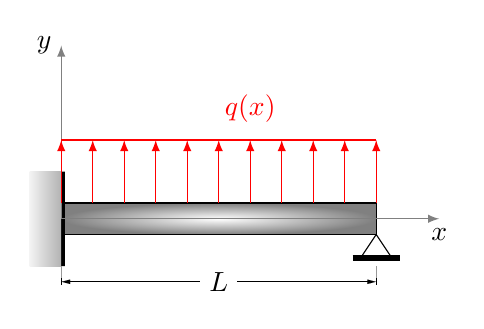
\begin{tikzpicture}[scale=4]
		% Viga
		\draw[outer color=gray, inner color=white] (0, -.1) rectangle (1, 0);
		
		% Apoyos
		\draw[line width=3pt] (0, -.2) rectangle (0, .1);
		\shade[left color=gray!10, right color=gray!60] (-.1, -.2) rectangle (0, .1);
		\draw[] (1, -.1) -- (1.05, -.175) -- (.95, -.175) -- cycle;
		\draw[line width=2pt] (.925, -.175) -- (1.075, -.175);
		
		% Ejes
		\draw[-latex, gray] (0,-.05) -- (1.2, -.05) node[below, black] {$x$};
		\draw[-latex, gray] (0,-.05) -- (0, .5) node[left, black] {$y$};
		
		% Cotas
		\dimline[extension start length=-.05, extension end length=-.05] {(0, -.25)} {(1, -.25)} {$L$};
		
		% Carga
		\foreach \x in {0, .1, ..., 1.01}{
		\draw[latex-, yscale=.4, red] (\x, .5) -- (\x, 0);}
		\draw[red, yscale=.4] (0, 0) -- (0, .5) -- (1, .5);
		\node[red] at (.6, .3) {$q(x)$};
	\end{tikzpicture}
\end{document}